\documentclass[11pt]{article}
%\usepackage{uvatoc} % replace this line with the one below for your submission
\usepackage[response]{uvatoc}

\newcommand{\one}{{\sf 1}}
\newcommand{\zero}{{\sf 0}}


\begin{document}

\makeheader

\makemytitle{Week 8: Turing Time}
\submitter {Benjamin (aqn9yv, dlb2ru, ht6xd, iad4de, jmn4fms, lw7jz)}

\directions{
\collaboration{You should work on the problems yourself, before discussing with
others, and with your cohorts are your cohort meeting. By the Assessed Cohort Meeting,
you and all of your cohortmates, should be prepared to present and discuss solutions to
all of the assigned problems (including the programming problems). In addition to discussing with your cohortmates, you may
discuss the problems with anyone you want, and use any resources you want except for
any materials from previous offerings of this course, which are not permitted.
You should document any resources you use (beyond the provided course materials) in your problem write-up.
}
}



\begin{problem}
Turing Machine for Majority
\end{problem}
\directions{
In the \href{https://www.youtube.com/watch?v=wN5DPmz0hgg}{\em Turing Machine Examples} video we begin but do not complete an ``Accept/Reject'' Turing machine for computing Majority (i.e., for a given input bit string, are there more \one s than \zero s?). The behavior of the Turing Machine is as follows (note that this description roughly matches the expected level of specificity of Turing Machine descriptions):
\begin{enumerate}
    \item Start from the beginning of the tape where a ``start of tape'' symbol (the $\triangle$) precedes the input 
    \item Move right through the tape, looking for a \zero.
    \item If a \zero\ is found, write over it with an $x$, then go back to the $\triangle$ (start of tape)
    \item Move right through tape, looking for a \one.
    \item If a \one\ is found, write over it with an $x$, then go back to the $\triangle$ (start of tape)
    \item Repeat the "look for \zero, mark if found, look for \one, mark if found" steps until a blank cell (the $\null$ symbol) is reached (meaning there are either no more \zero s or no more \one s)
    \item Go back to the beginning of the tape, looking for \one s
    \item if a \one\ is found along the way, return 1. Otherwise, return 0.
\end{enumerate}

The following image depicts one potential implementation of the machine described above:

\begin{center}
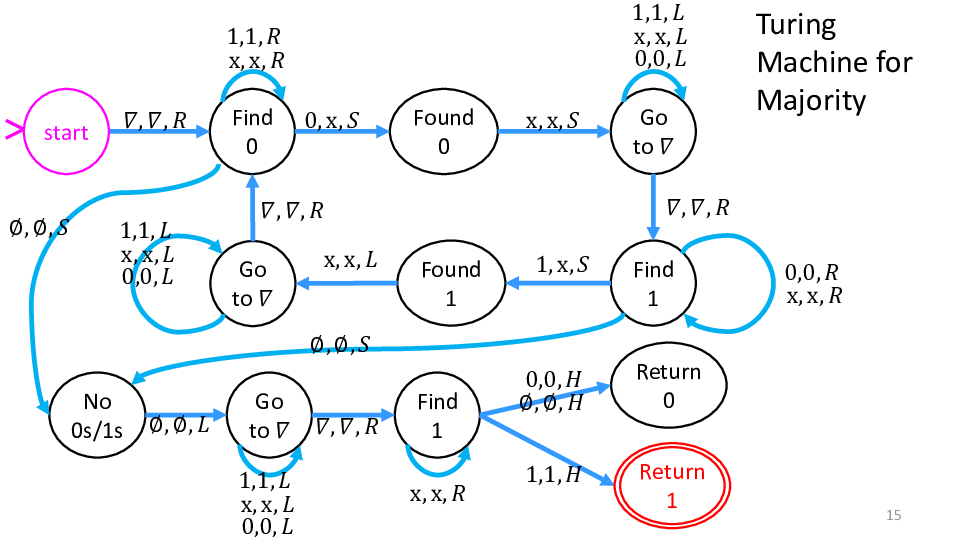
\includegraphics[scale=0.5]{maj_machine.png}
\end{center}

In this machine, each transition is a triple, where the first value is the symbol read from the tape when taking that transition, the second is the symbol to write onto the tape in its place, and the third symbol is a control instruction ($L$ for move left in the tape, $R$ for move right in the tape, $S$ for stay put in the tape, and $H$ for halt).

Consider that this machine is given each of the inputs describe below, all of which are $n$ bits long. Give a $\Theta$ bound on the total number of transitions this machine would take before halting as a function of the input length $n$.

\begin{enumerate}[a.]
    \item A string of $n$ \one s
    \item A string of $n$ \zero s
    \item A string of $\frac{n}{2}$ copies of \zero\one pairs (e.g. \zero\one\zero\one\zero\one...). You may assume $n$ is even.
    \item A \one followed by $\frac{n-1}{2}$ copies of \zero\one pairs (e.g. \one\zero\one\zero\one\zero\one...). You may assume $n$ is odd.
\end{enumerate}
}

\begin{enumerate}[a.]
\item $\Theta(n): f_{a}(n) = 2n + 5$ 

Since everything on the tape is 1, the machine will look for 0s for n transitions, in vain, and take n more steps to go back beginning. It will then start looking for uncrossed 0, which occurs at its first step. Several constant transitions are added. 
\begin{figure}[ht!]
  \centering
  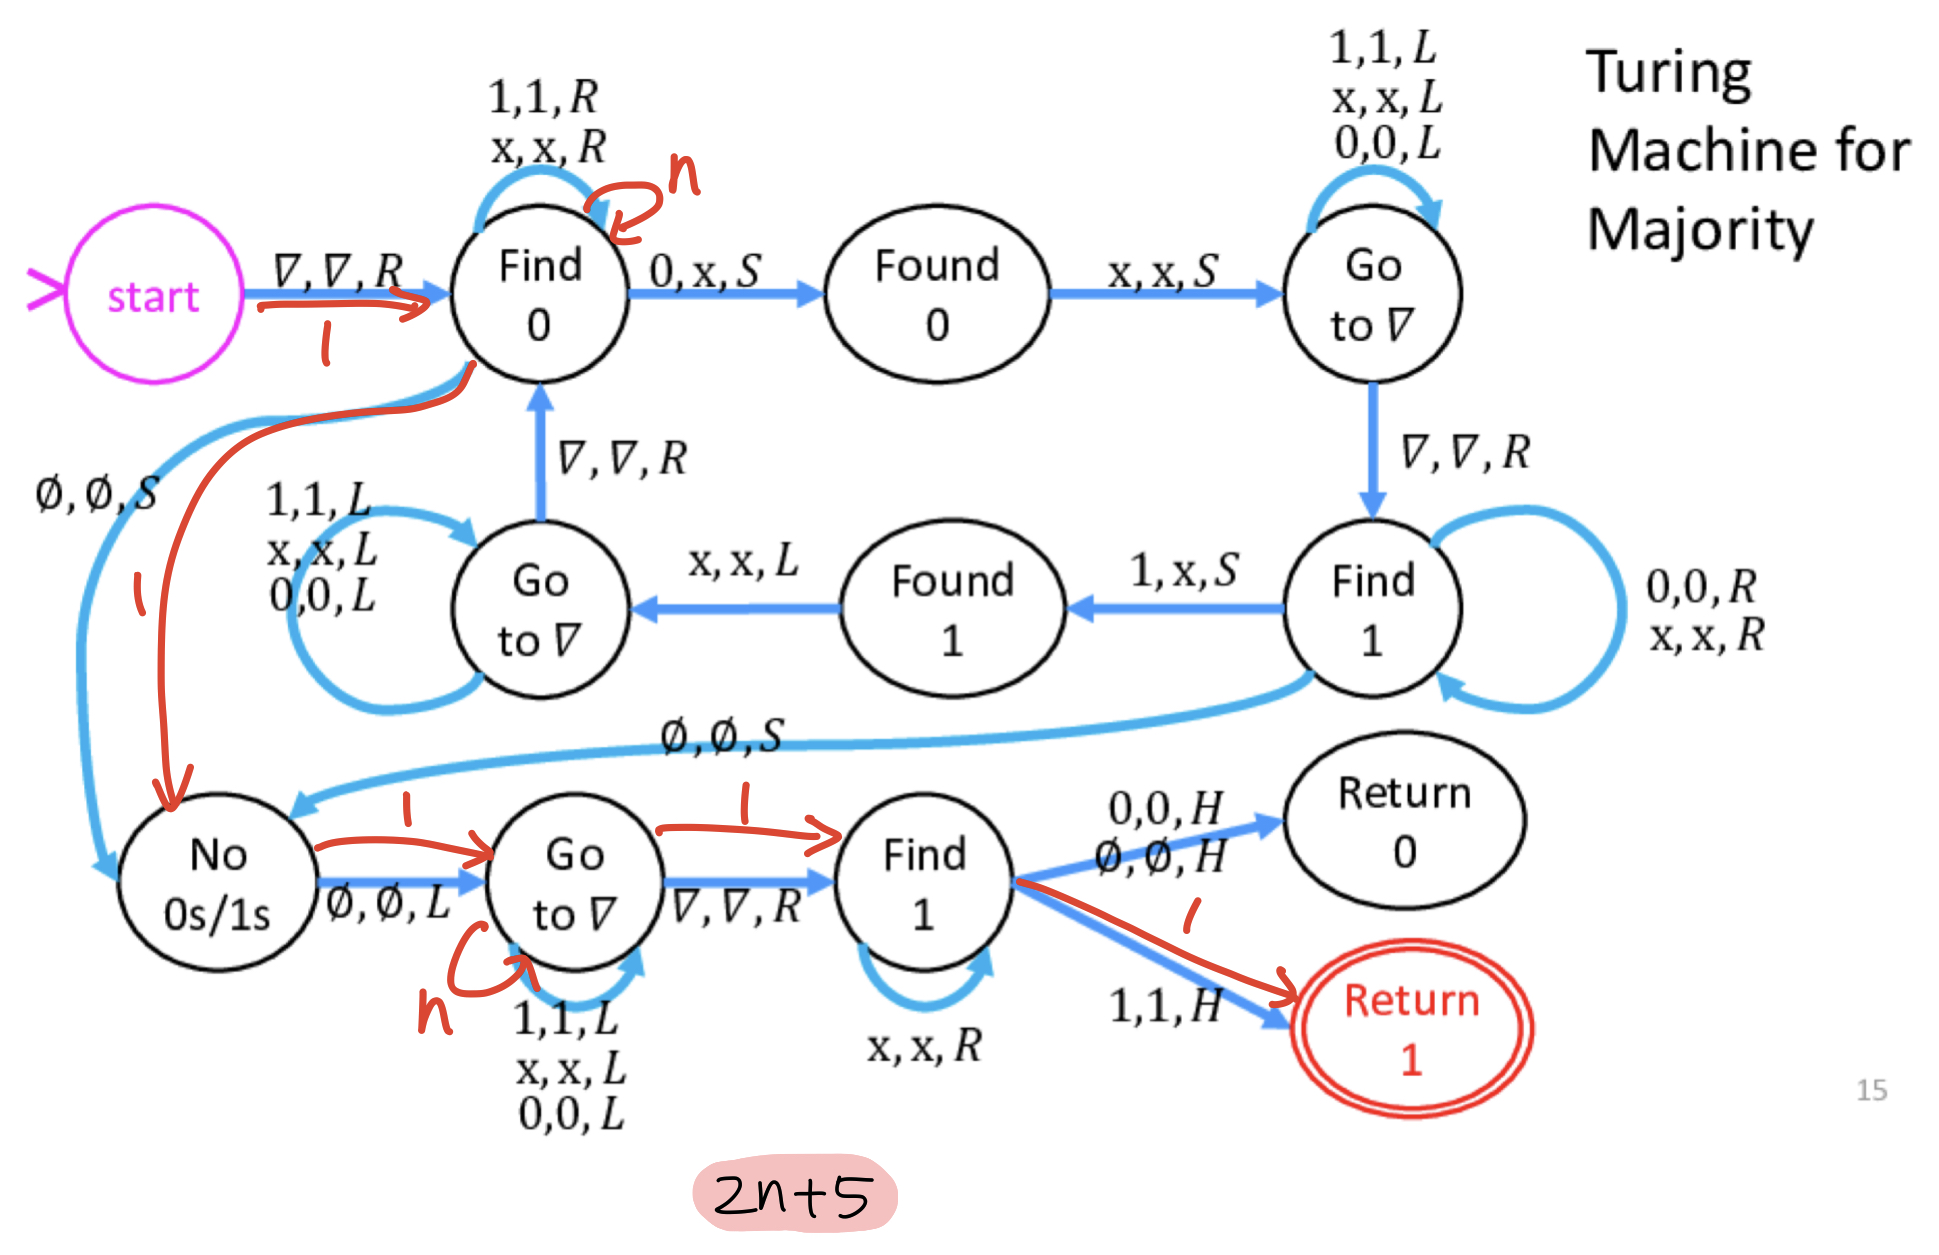
\includegraphics[origin=c, height=60mm]{1.jpeg}
\end{figure}

\item $\Theta(n): f_{b}(n) = 2n + 9$

Since everything on the tape is 0, the machine will find a first 0 and then go back beginning. Then it starts looking for 1s for n transitions, in vain, and takes n more steps to go back beginning. It will then start looking for uncrossed 1, which occurs at its first step. Several constant transitions are added. 
\begin{figure}[ht!]
  \centering
  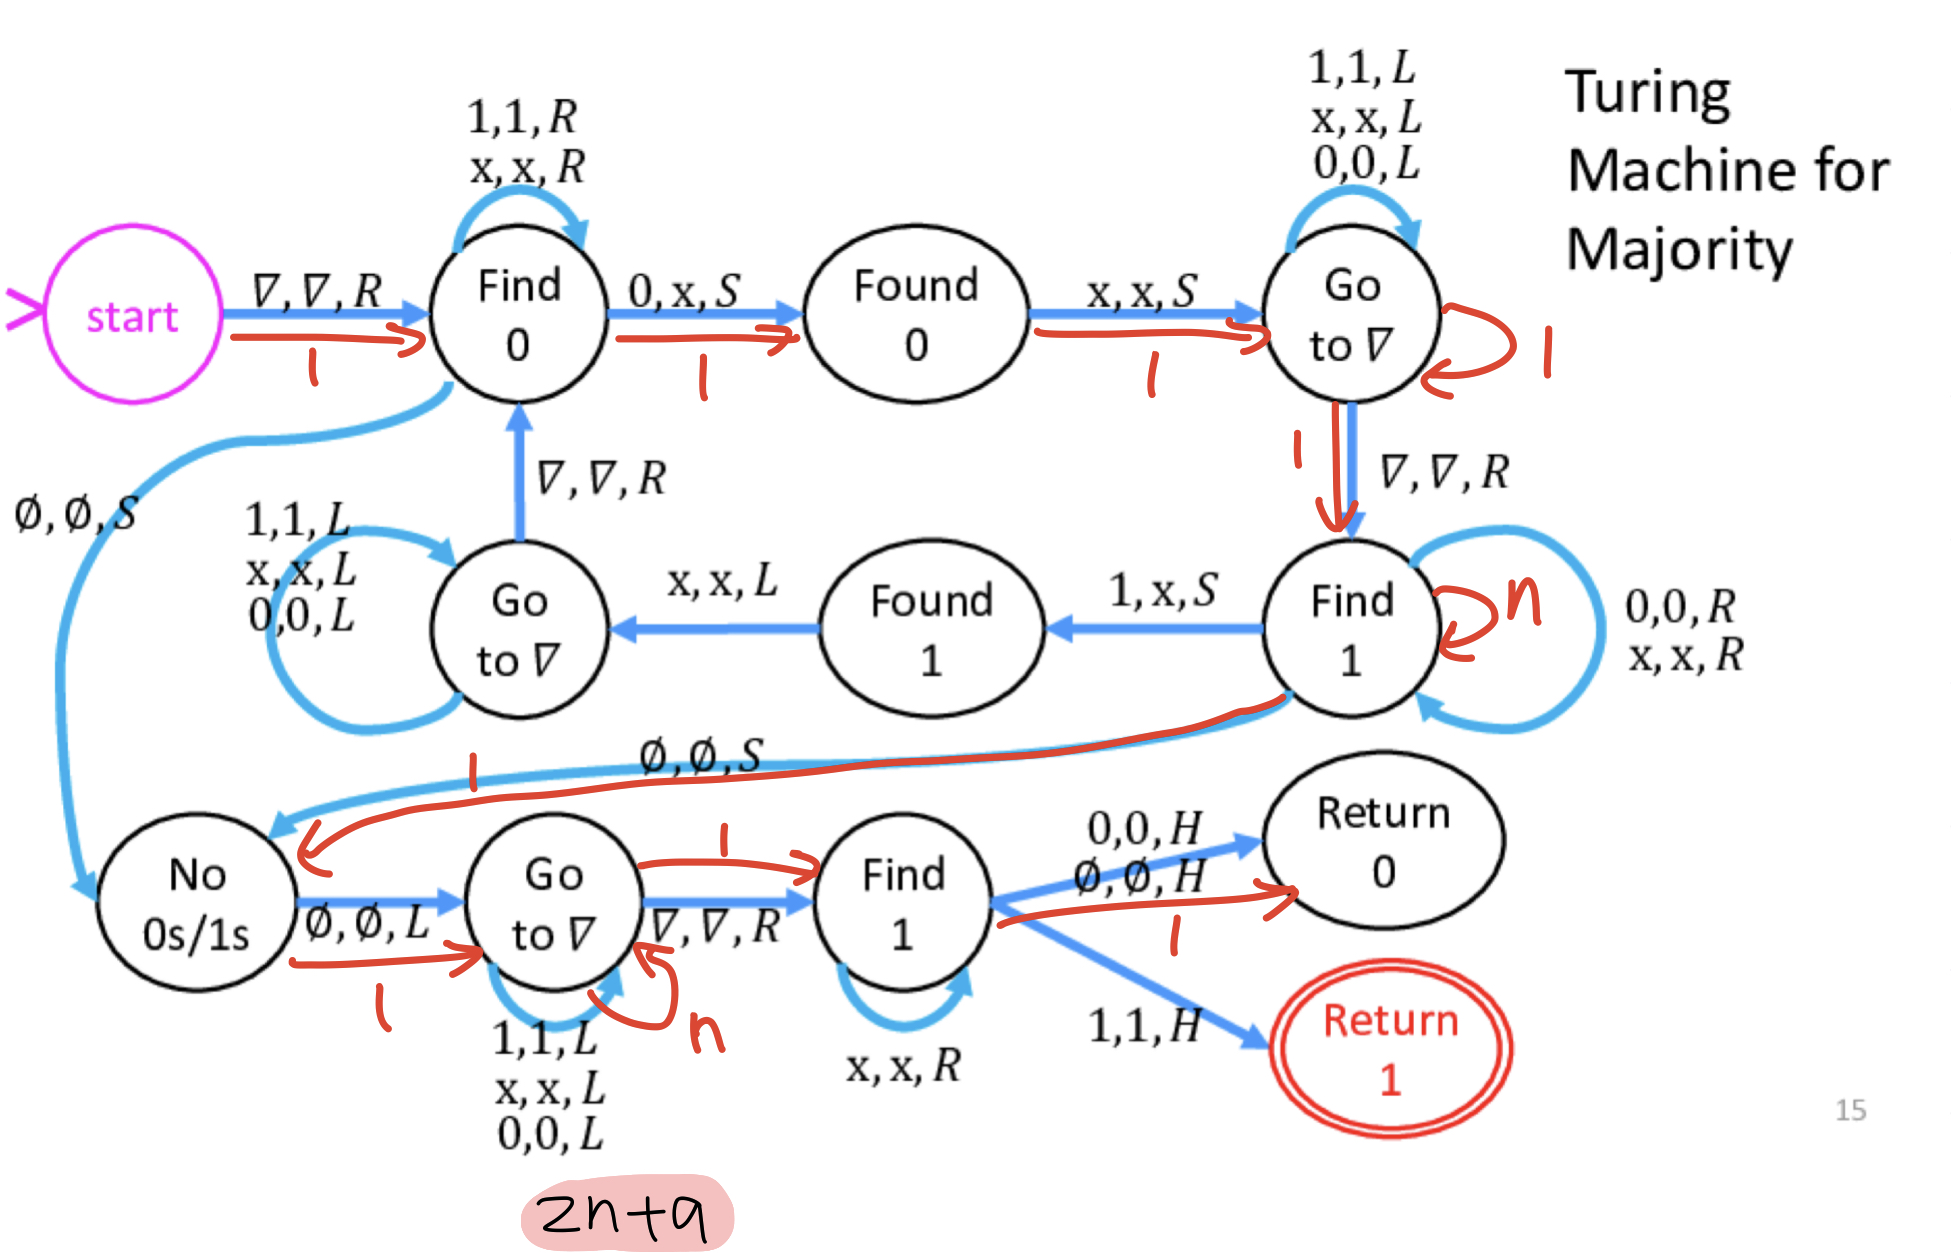
\includegraphics[origin=c, height=60mm]{2.jpeg}
\end{figure}

\item $\Theta(n^2): f_{c}(n) = 2n^2 + 9n + 5$ 

Since tape reads 010101..., the machine will look for 0s and 1s in turn, each turn averaging $\frac{n}{2}$ transitions. This number is doubled by including steps go back beginning after each turn. After n turns, it will start again looking for more 0s for n transitions, in vain, and takes n more steps back to beginning. It will then start looking for uncrossed numbers in vain, taking n more steps. Several constant transitions are added.
\begin{figure}[ht!]
  \centering
  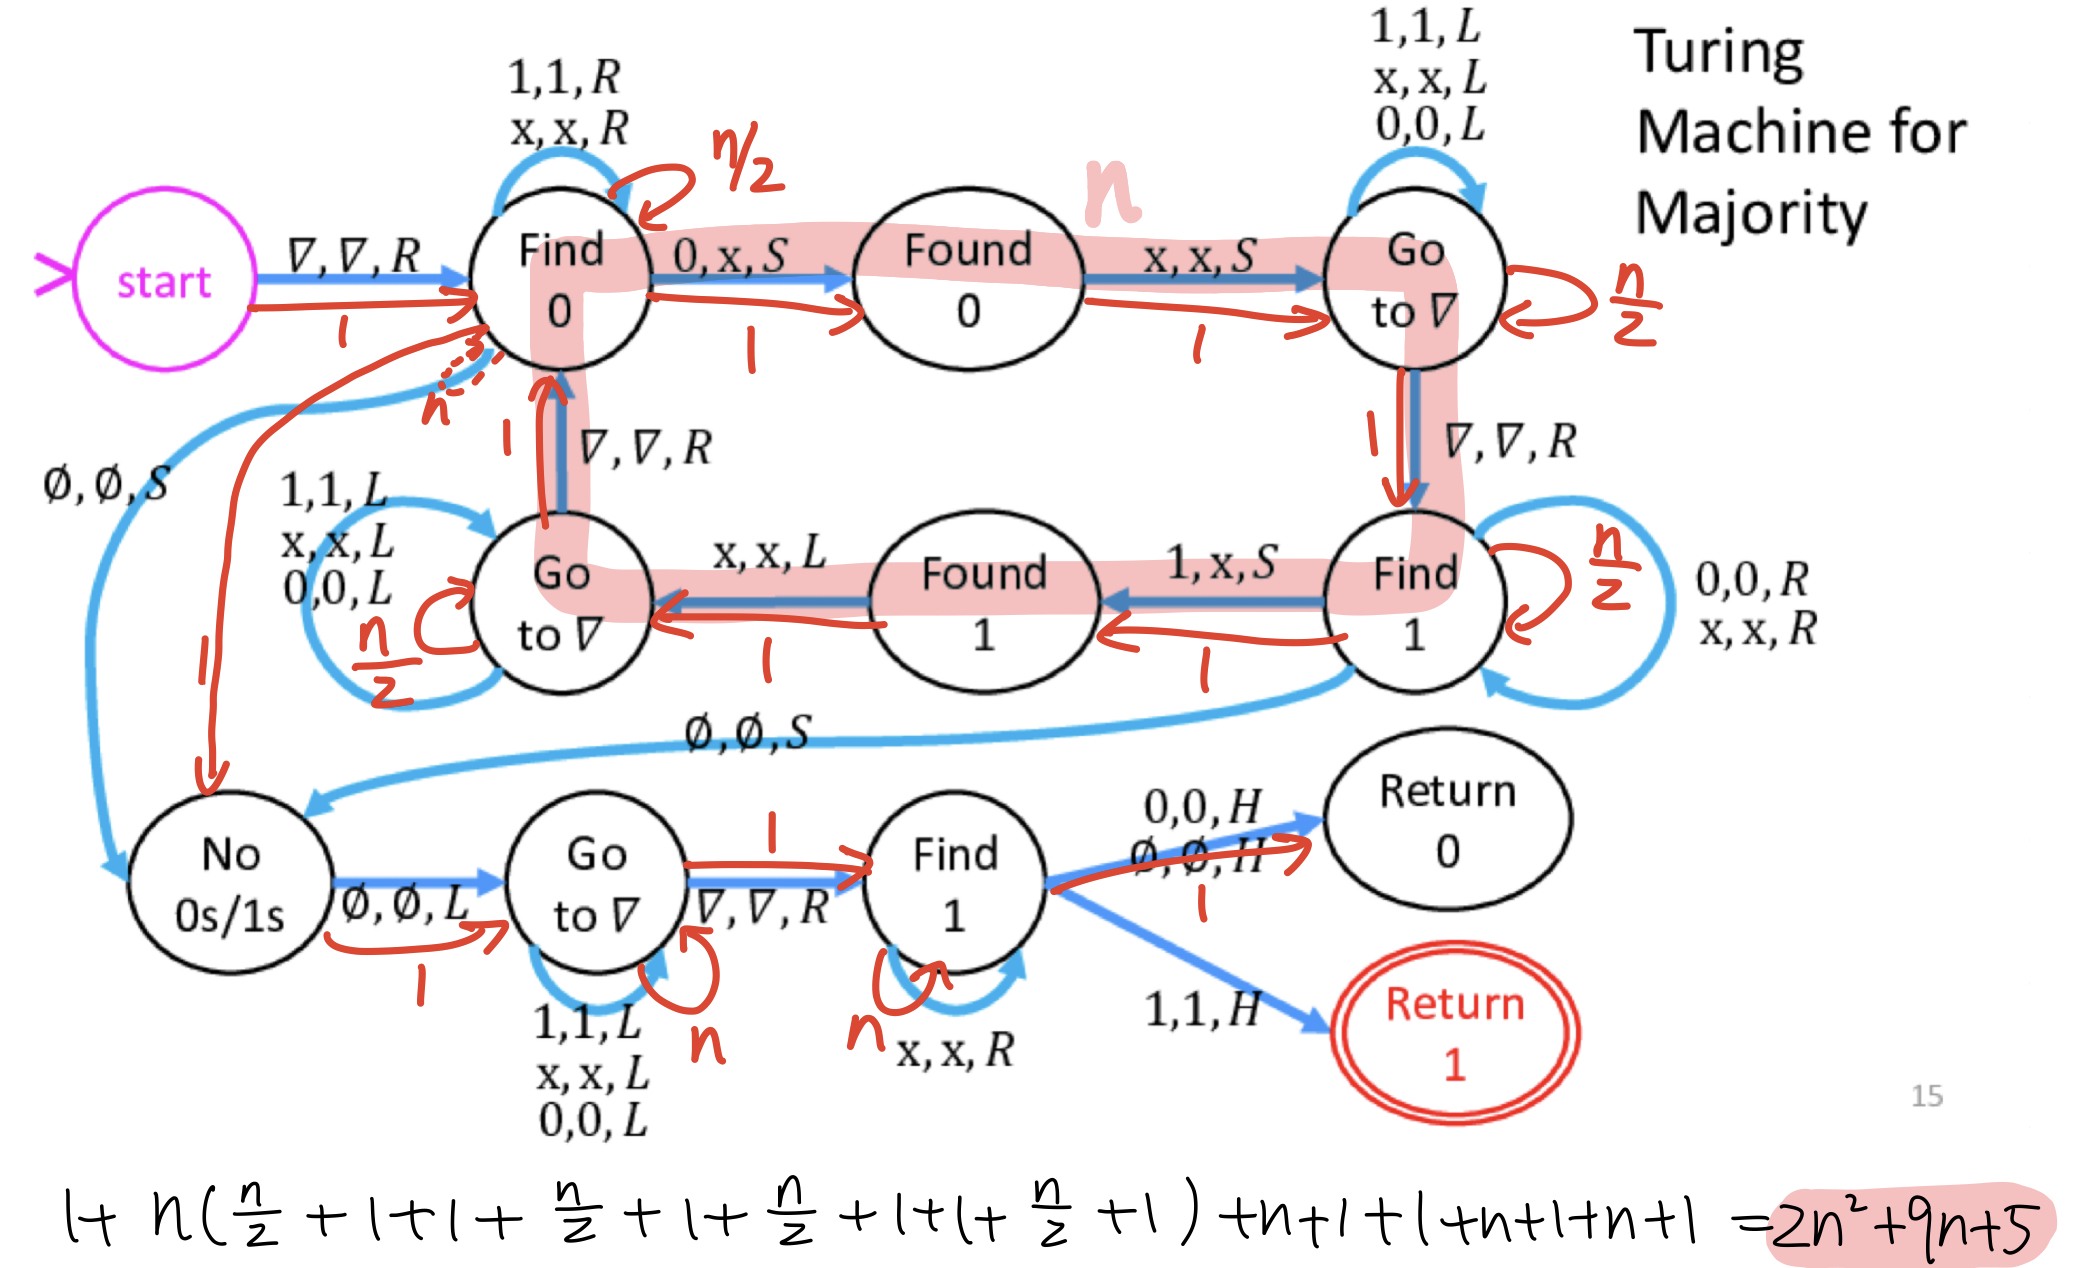
\includegraphics[origin=c, height=70mm]{3.jpeg}
\end{figure}

\item $\Theta(n^2): f_{d}(n) = 2n^2 + 9n + 4$ 

Since tape reads 1010101..., the machine will look for 1s and 0s in turn, each turn averaging $\frac{n}{2}$ transitions. This number is doubled by including steps go back beginning after each turn. After n turns, it will start again looking for more 0s for n transitions in vain, and takes n more steps back to beginning. It will then start looking for uncrossed 1, taking n-1 more steps to find the last 1. Several constant transitions are added.
\begin{figure}[ht!]
  \centering
  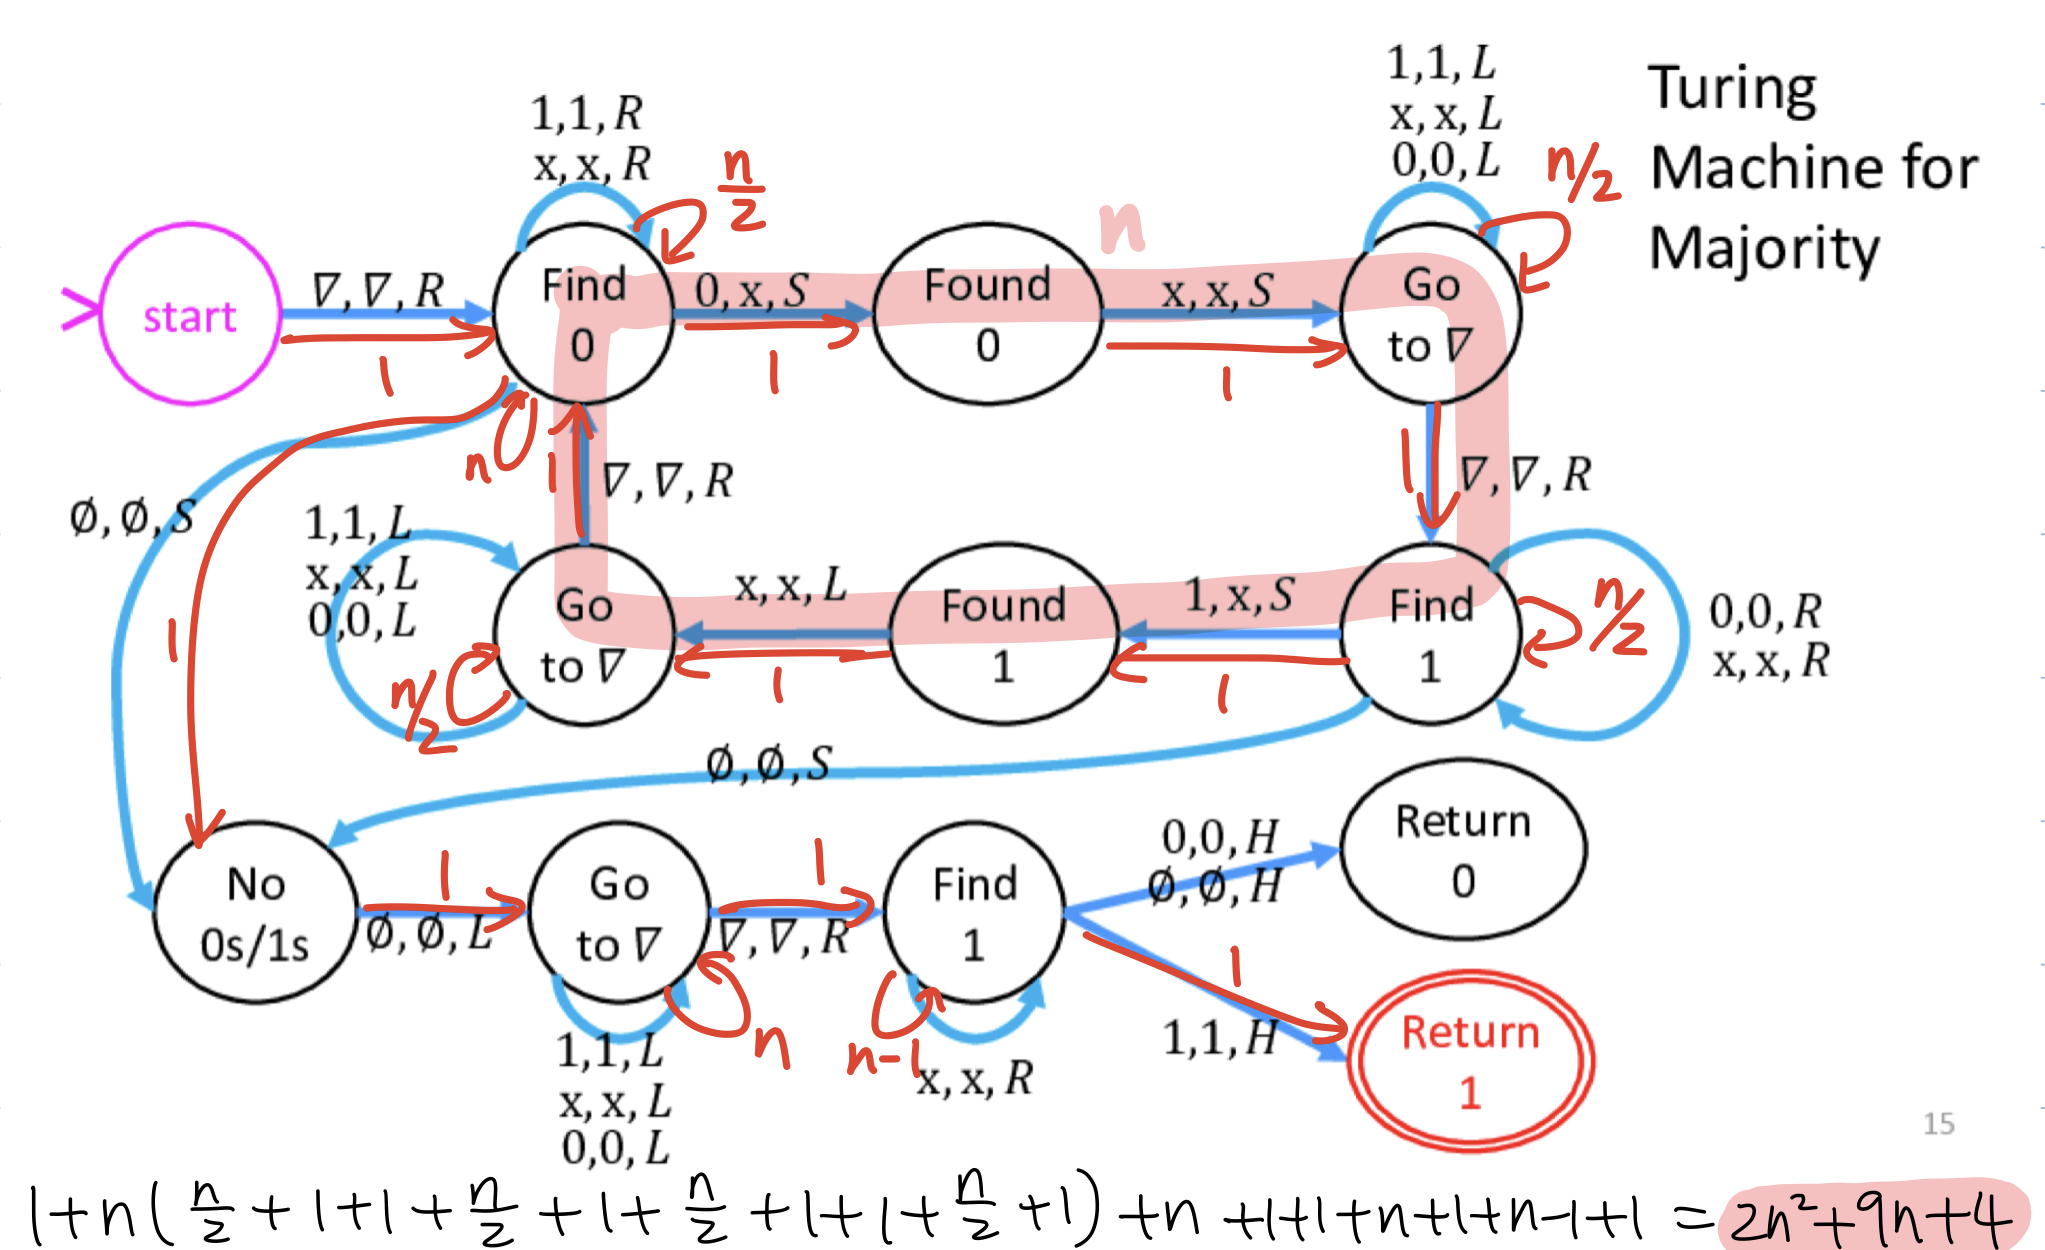
\includegraphics[origin=c, height=70mm]{4.jpeg}
\end{figure}

\end{enumerate}

\end{document}
